\chapter{Decision tree induction as solving an MDP}\label{sec:dt-mdp}

\section{The Markov decision process}\label{sec:the-mdp}
We now formulate the decision tree induction problem (cf. definition~\ref{eq:suplearning}) as finding the optimal policy in an MDP (cf. definition~\ref{def:mdp-obj}).
Given a set of examples $\mathcal{E}$, the induction of a decision tree is made of a sequence of decisions: at each node, we must decide whether it is better to split (a subset of) $\mathcal{E}$, or %assign a class label and 
to create a leaf node.
This sequential decision-making process corresponds to an MDP $\mathcal{M} \langle S, A, R_{\alpha}, T, T_0 \rangle$ (cf. definition~\ref{def:mdp}) that we present next.
A state is a pair made of a subset of examples $\mathcal{X}\subseteq\mathcal E$ and a depth $d$.
Like for classification POIBMDPs (cf. definition~\ref{def:ibmdp} and algorithm~\ref{alg:extract-tree}), the depth $d$ is actually not necessary to extract a tree from a policy.
However, it is necessary in order to solve the MDP.
Indeed, because we constrain the model class to limited-depth trees, the horizon of our MDP is finite and hence as per~\cite{puterman}, the optimal policy is non-Markovian and depends on the time.

The set of states is $S = \{ (\mathcal{X}, d) \in P(\mathcal{E}) \times \{0, \ldots, D\} \}$ where $P(\mathcal{E})$ denotes the power set of $\mathcal{E}$. $d \in \{0,\ldots,D\}$ is the current depth in the tree.
An action $A$ consists in creating either a split node, or a leaf node (label assignment). We denote the set of candidate split nodes $ {\mathcal F} $. A split node in $\mathcal F$ is a pair made of one feature $i$ and a threshold value $x_{ij}\in \mathcal{E}$.
So, we can write $A = {\mathcal{F} \cup \{ 1, \ldots, K \}}$ (these are essentially information gathering actions).
From state $s=(X,d)$ and a splitting action $a \in {\mathcal F}$, the transition function $P$ moves to the next state $s_l = (\mathcal{X}_l, d+1)$ with probability $p_l = \frac{|\mathcal{X}_l|}{|\mathcal{X}|}$ where $\mathcal{X}_l = \{(\boldsymbol{x}_i, y_i) \in \mathcal{X}: \boldsymbol{x}_i \leq x_{ij}\}$, or to state $s_r = (\mathcal{X} \setminus \mathcal{X}_l, d+1)$ with probability $1-p_l$. For a class assignment action $a \in \{1,\ldots,K\}$, the chain reaches an absorbing terminal state with probability 1. 
The reward function $R_{\alpha}: S \times A \rightarrow \mathbb{R}$ returns $-\alpha$ for splitting actions (this is $\zeta$ in a classification POIBMDP (cf. definition~\ref{def:cpoibmdp})) and the proportion of misclassified examples of $\mathcal{X}$ $-\frac{1}{|\mathcal{X}|}\sum_{(\boldsymbol{x}_i,y_i) \in \mathcal{X}} l(y_i, a)$ for class assignment actions. $\alpha \in [0,1]$ controls the accuracy-complexity trade-off defined in the regularized training objective \ref{eq:suplearning}. 

The solution to this MDP is a deterministic policy $\pi: S \rightarrow A$ that maximizes {$J_{\alpha}(\pi) ={\mathbb{E}}\left[\sum_{t = 0}^D R_{\alpha}(s_t, \pi(s_t))\right]$\label{def:finite-mdp-obj}}, the expected sum of rewards where the expectation is taken over transitions $s_{t+1}\sim P(s_t, \pi(s_t))$ starting from initial state $s_0 = (\mathcal{E}, 0)$.
This objective is a re-writing of the RL objective (cf. definition~\ref{def:mdp-obj}) where the trajectory have finite lengths $D$ rather than being infinite.
Any such policy can be converted into a binary decision tree through a recursive extraction function $E(\pi, s)$ (equivalent to algorithm~\ref{alg:extract-tree}) that returns, either a leaf node with class $\pi(s)$ if $\pi(s)$ is a class assignment, or a tree with root node containing split $\pi(s)$ and left/right sub-trees $E(\pi, s_l)$/$E(\pi, s_r)$ if $\pi(s)$ is a split. The final decision tree $T$ is obtained by calling $E(\pi, s_0)$ on the initial state $s_0$. 

\begin{proposition}[Objective Equivalence]\label{prop:equiv}
Let $\pi$ be a deterministic policy of the MDP (cf. section~\ref{sec:the-mdp}) and $\pi^*$ be an optimal deterministic policy. 
Then $J_\alpha(\pi) = -{\mathcal L}_\alpha(E(\pi, s_0))$ and $T^* = E(\pi^*, s_0)$ where $T^*$ is a tree that optimizes the decision tree induction objective (cf. definition~\ref{eq:suplearning}).
\end{proposition}
This proposition is key as it states that the return of any policy of the MDP defined above is equal to the regularized training accuracy of the tree extracted from this policy.
A consequence of this proposition is that when all possible splits are considered, the optimal policy will generate the optimal tree w.r.t the decision tree induction objective.

\begin{proof}
For the purpose of the proof, we overload the definition of $J_\alpha$ and $\mathcal L_\alpha$, to make explicit the dependency on the dataset and the maximum depth. 
As such, $J_\alpha(\pi)$ becomes $J_\alpha(\pi, {\mathcal E}, D)$ and ${\mathcal L}_\alpha(T)$ becomes ${\mathcal L}_\alpha(T, {\mathcal E})$. 
Let us first show that the relation $J_\alpha(\pi, {\mathcal E}, 0) = -{\mathcal L}_\alpha(T, {\mathcal E})$ is true. 
If the maximum depth is $D = 0$ then $\pi(s_0)$ is necessarily a class assignment, in which case the expected number of splits is zero and the relation is obviously true since the reward is the opposite of the average classification loss. 
Now assume it is true for any dataset and tree of depth at most $D$ with $D \geq 0$ and let us prove that it holds for all trees of depth $D + 1$. 
For a tree $T$ of depth $D + 1$ the root is necessarily a split node. Let $T_l = E(\pi, s_l)$ and $T_r = E(\pi, s_r)$ be the left and right sub-trees of the root node of $T$. 
Since both sub-trees are of depth at most $D$, the relation holds and we have $J_\alpha(\pi, \mathcal{X}_l, D) = {\mathcal L}_\alpha(T_l, \mathcal{X}_l)$ and $J_\alpha(\pi, \mathcal{X}_r, D) = {\mathcal L}_\alpha(T_r, \mathcal{X}_r)$, where $\mathcal{X}_l$ and $\mathcal{X}_r$ are the datasets of the ``right'' and ``left'' states to which the MDP transitions---with probabilities $p_l$ and $p_r$---upon application of $\pi(s_0)$ in $s_0$, as described in the MDP formulation. 
Moreover, from the definition of the policy return we have 
\begin{align*}
   J_\alpha(&\pi, {\mathcal E}, D + 1) = -\alpha + p_l * J_\alpha(\pi, \mathcal{X}_l, D) + p_r * J_\alpha(\pi, \mathcal{X}_r, D)\\
   &= -\alpha - p_l * {\mathcal L}_\alpha(T_l, \mathcal{X}_l) - p_r * {\mathcal L}_\alpha(T_r, D)\\
   &= -\alpha - p_l * \Bigg(\frac{1}{|\mathcal{X}_l|}\sum_{(\boldsymbol{x}_i, y_i)\in \mathcal{X}_l}l(y_i, T_l(\boldsymbol{x}_i))  + \alpha C(T_l)\Bigg)\\
   &\ - p_r * \Bigg(\frac{1}{|\mathcal{X}_r|}\sum_{(\boldsymbol{x}_i, y_i)\in \mathcal{X}_r}l(y_i, T_r(\boldsymbol{x}_i))  + \alpha C(T_r)\Bigg)\\
   &= -\frac{1}{N}\sum_{(\boldsymbol{x}_i, y_i)\in \mathcal{X}}l(y_i, T(\boldsymbol{x}_i)) - \alpha (1 + p_l C(T_l) + p_r C(T_r))\\
   &= -{\mathcal L}(T, {\mathcal E}) 
\end{align*}
\end{proof}

\section{Algorithm}\label{sec:dpdt}

We now present the Dynamic Programming Decision Tree (DPDT) induction algorithm. 
The algorithm consists of two essential steps. The first and most computationally expensive step constructs the MDP presented in section~\ref{sec:the-mdp}. 
The second step solves it to obtain a policy that maximizes the objective from definition~\ref{def:finite-mdp-obj} and that is equivalent to a decision tree. Both steps are now detailed.

\subsection{Constructing the MDP}

An algorithm constructing the MDP of section~\ref{sec:the-mdp} essentially computes the set of all possible decision trees of maximum depth $D$ which decision nodes are in $\mathcal F$. 
The transition function of this specific MDP is a directed acyclic graph. Each node of this graph corresponds to a state for which one computes the transition and reward functions. 
%% PP : je comment-out ce qui suit qui est un detail d'implantation qui ne change rien à la complexité de l'algorithme. Il faut le dire plus loin ; d'ailleurs il en est aussi déjà question en 4.3.
%To limit memory usage of non-terminal nodes, instead of storing all the samples in $(\mathcal{X},d)$, we only store $d$ and the binary vector of size $N$, $x_{bin} = {(1_{\{\boldsymbol{x}_i \in \mathcal{X}\}})}_{i\in \{1,\ldots,N\}}$. 
%Even then,
Considering all possible splits in $\mathcal F$ does not scale.
We thus introduce a state-dependent action space $A_s$, much smaller than $A$ and populated by a splits generating function. In figure \ref{fig:schema-mdp}, we illustrate the MDP constructed for the classification of a toy dataset using some arbitrary splitting function.

\begin{figure}
      \centering
      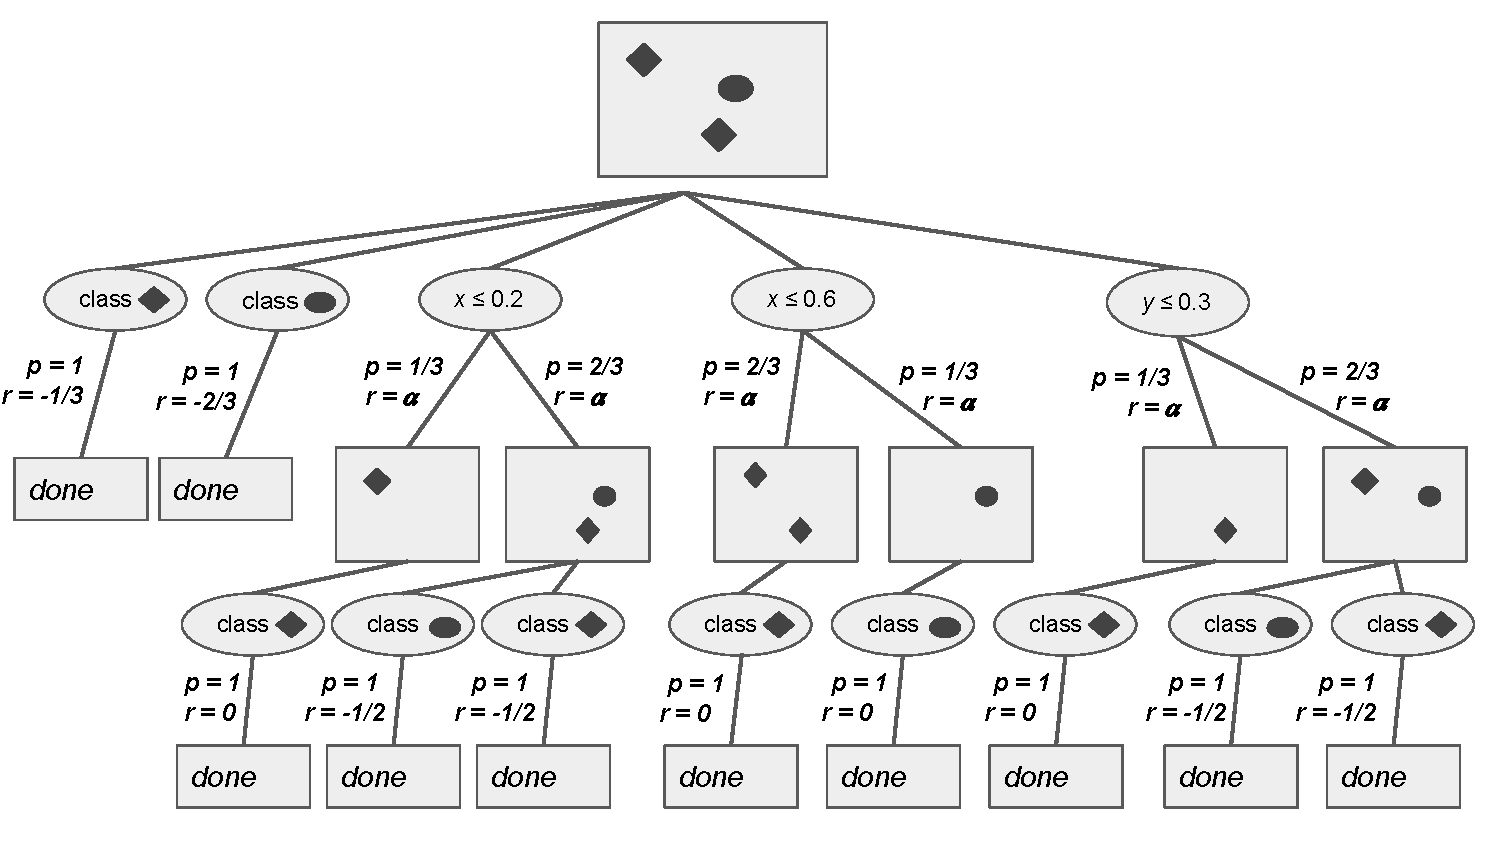
\includegraphics[width=0.9\linewidth]{images/figures/schema_mdp.pdf}
      \caption{Schematics of the MDP from section~\ref{sec:the-mdp} to learn a decision tree of depth 2 to classify a toy dataset with three samples, two features (x,y), and two classes (oval, diamond) and using an arbitrary splits generating function.}\label{fig:schema-mdp}
      \end{figure}

\subsection{Heuristic splits generating functions}\label{sec:testgen}

A split generating function is any function $\phi$ that maps an MDP state, i.e., a subset of training examples, to a split node. It has the form $\phi: S \rightarrow P(\mathcal{F})$, where $P(\mathcal{F})$ is the power set of all possible split nodes in $\mathcal F$. 
For a state $s \in S$, the state-dependent action space is defined by $A_s = \phi(s) \cup  \{1,\ldots,K\}$. 

When the split generating function does not return all the possible candidate split nodes given a state, solving the MDP with state-dependent actions $A_s$ is not guaranteed to yield the minimizing tree for the decision tree induction problem (cf. definition~\ref{eq:suplearning}), as the 
optimization is then performed on the subset of trees of depth smaller or equal to $D$, $\mathcal{T}_D$. 
We now define some interesting split generating functions and provide the time complexity of the associated decision tree algorithms. The time complexity is given in big-O of the number of candidate split nodes considered during computations. 
% Building a depth-1 greedy tree hides a time complexity of $O(np\log(np))$ to sort the splits by information gains \cite{breiman1984classification}.
%%%>>>>>>> c90c7909bd5d3b8cfee3901e21a456980dfd72e1

\paragraph{Exhaustive function} When $\mathcal{F} \subseteq \phi(s), \forall s \in S$, the MDP contains all possible splits of a certain set of examples. In this case, \textit{the optimal MDP policy is the optimal decision tree of depth at most D},
and the number of states of the MDP would be $O({(2Np)}^D)$. Solving the MDP for $A_s = \phi(s)$ is equivalent to running one of the optimal tree induction algorithms~\cite{verwer2017learning,oct,pystreed,quantbnb,binoct,murtree,mfoct,blossom,lin2020generalized,chaouki2024branchesfastdynamicprogramming}.

\paragraph{Top $B$ most informative splits}\label{topk-heuristic}~\cite{topk} proposed to generate splits with a function that returns, for any state $s=(\mathcal{X},d)$, the $B$ most informative splits over $\mathcal{X}$ with respect to some information gain measure such as the entropy or the Gini impurity. 
The number of states in the MDP would be $O({(2B)}^D)$. \textit{When $B=1$, the optimal policy of the MDP is the greedy tree.} 
In practice, we noticed that the returned set of splits lacked diversity and often consists of splits on the same feature with minor changes to the threshold value. 

% PP : don't know why mais ci-dessous, si on met un '.' après {CART}, le pdf en affiche 2. Si on n'en met pas, on en voit un !
\paragraph{Calls to CART}\label{cart-heuristic} Instead of returning the most informative split at each state $s=(\mathcal{X},d)$, we propose to find the most discriminative split, i.e.\@ the feature splits that best predicts the class of data in $\mathcal{X}$.
We can do this by considering the split nodes of the greedy tree. In practice, we run CART on $s$ and use the returned nodes as $\phi(s)$. We control the number of MDP states by constraining CART trees with a maximum number of nodes $B$: $\phi(s) = nodes(\text{CART}(s, max\_nodes=B))$
The number of MDP states would be $O({(2B)}^D)$.\textit{When $B=1$, the MDP policy corresponds to the greedy tree.} The process of generating split nodes with calls to CART is illustrated in figure \ref{fig:schema-dpdt}.

\begin{figure}
      \centering
      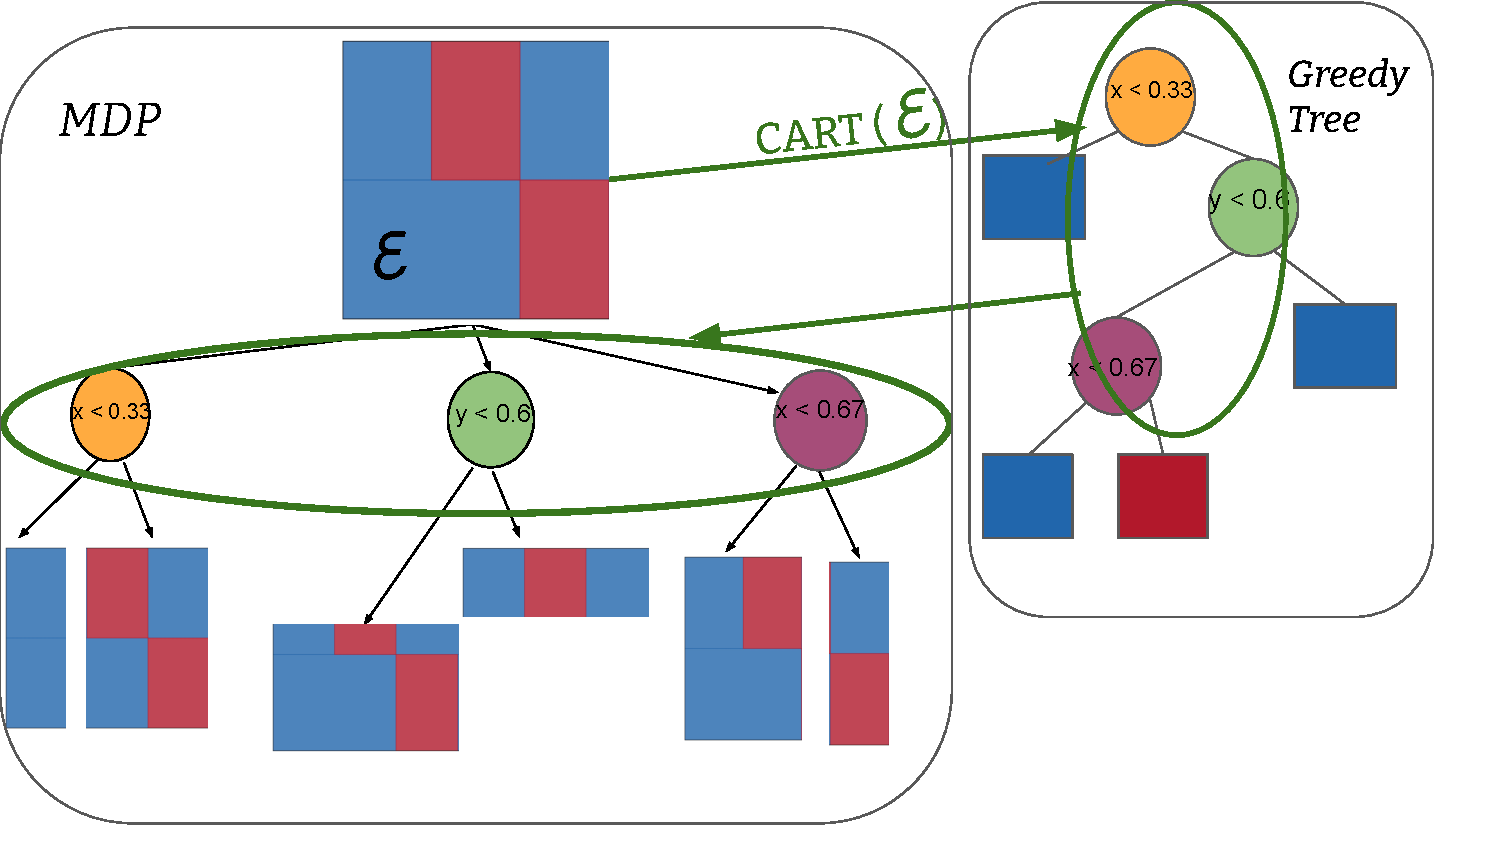
\includegraphics[trim={0 0cm 0 0},clip,width=0.9\textwidth]{images/figures/schematic_cart_node_select.pdf}
      \caption{How CART is used in DPDT to generate candidate splits given the example data in the current state.}\label{fig:schema-dpdt}
\end{figure}



\subsection{Dynamic programming to solve the MDP}
\RestyleAlgo{ruled}
\SetKwComment{Comment}{}{}
        \begin{algorithm}
            \KwData{$\text{Dataset }\mathcal{E}, \text{max depth }D, \text{split function }\phi(), $\\
            $\text{split function parameter } B,  \text{regularizing term }\alpha$}
            \KwResult{$\text{Tree } T$}
            $\mathcal{M} \gets build\_mdp(\mathcal{E}, D, \phi(), B)$\label{line:build_mdp} \\
            \Comment{{// Backward induction}}
            $Q^*(s,a) \gets R_{\alpha}^{\mathcal{M}}(s,a) + \sum_{s'} P^{\mathcal{M}}(s,a,s') \max_{a' \in A_{s'}^{\mathcal{M}}} Q^*(s',a') \forall s,a \in \mathcal{M}$\\
            \Comment{{// Get the optimal policy}}
            $\pi^*(s) = \operatorname{argmax}_{a \in A_s^{\mathcal{M}}} Q^*(s, a) \forall s \in \mathcal{M} $\\
            \Comment{{// Extracting tree from policy}}
            $T \gets E(\pi^*,s_0^{\mathcal{M}}) $
            \caption{DPDT}\label{alg:dpdt}
        \end{algorithm}
        
After constructing the MDP with a chosen splits generating function, we solve for the optimal policy using dynamic programming. Starting from terminal states and working backward to the initial state, we compute the optimal state-action values using Bellman's optimality equation~\cite{Bellman}, and then deducing the optimal policy.

From now on, we write DPDT to denote algorithm \ref{alg:dpdt} when the split function is a call to CART. We discuss key bottlenecks when implementing DPDT in subsequent sections. We now state theoretical results when using DPDT with the CART heuristic. 

\subsection{Performance guarantees for DPDT}
We now show that: 1) DPDT minimizes the loss from decision tree induction objective (cf. definition~\ref{eq:suplearning}) at least as well as greedy trees and 2) there exists problems for which DPDT has strictly lower loss than greedy trees. 
As we restrict the action space at a given state $s$ to a subset of all possible split nodes, DPDT is not guaranteed to find the tree minimizing Eq. \ref{eq:suplearning}. However, we are still guaranteed to find trees that are better or equivalent to those induced by CART:
\begin{theorem}[MDP solutions are not worse than the greedy tree]\label{prop:cart}
Let $\pi^*$ be an optimal deterministic policy of the MDP, where the action space at every state is restricted to the top $B$ most informative or discriminative splits. 
Let $T_0$ be the tree induced by CART and $\{T_1,\dots,T_M\}$ all the sub-trees of $T_0$, \footnote{These sub-trees are interesting to consider since they can be returned by common postprocessing operations following a call to CART, that prune some of the nodes from $T_0$. Please see \cite{pruning1} for a review of pruning methods for decision trees.} then for any $\alpha > 0$, 
\[
{\mathcal L}_\alpha(E(\pi^*, s_0)) \leq \min_{0\leq i\leq M}{\mathcal L}_\alpha(T_i)
\]
\end{theorem}

\begin{proof}
Let us first define $C(T)$, the expected number of splits performed by tree $T$ on dataset $\mathcal E$. 
Here $T$ is deduced from policy $\pi$, i.e. $T=E(\pi, s_0)$. $C(T)$ can be defined recursively as $C(T) = 0$ if $T$ is a leaf node, and $C(T) = 1 + p_l C(T_l) + p_r  C(T_r)$, where $T_l = E(\pi, s_l)$ and $T_r = E(\pi, s_r)$. 
In words, when the root of $T$ is a split node, the expected number of splits is one plus the expected number of splits of the left and right sub-trees of the root node.
\end{proof}

It is known that the greedy tree of depth 2 fails to perfectly classify the XOR problem as shown in figure \ref{fig:patho} and in \cite{Murthy,how-eff}. We aim to show that DPDT is a cheap way to alleviate the weaknesses of greedy trees in this type of problems. The following theorem states that there exist classification problems such that DPDT optimizes the regularized training loss strictly better than greedy algorithms such as CART, ID3 or C4.5.
\begin{theorem}[DPDT can be strictly better than greedy]\label{thm:better_greedy}
There exists a dataset and a depth $D$ such that the DPDT tree $T^{DPDT}_D$ is strictly better than the greedy tree $T^{greedy}_{D}$ , i.e, $\mathcal{L}_{\alpha=0}(T^{greedy}_{D}) > \mathcal{L}_{\alpha=0}(T^{DPDT}_{D})$.
\end{theorem}

The proof of this theorem is given in the next section.

\subsection{Proof of improvement over CART}\label{proof-improve-opt}
In this section we construct a dataset for which the greedy tree of depth 2 fails to accurately classify data while DPDT with calls to CART as a splits generating function guarantees a strictly better accuracy. The dataset is the XOR pattern like in figure \ref{fig:patho}. We will first show that greedy tree induction like CART chooses the first split at random and the second split in between the two columns or rows. Then we will quantify the misclassification of the depth-2 greedy tree on the XOR gate. Finally we will show that using the second greedy split as the root of a tree and then building the remaining nodes greedily, i.e. running DPDT with the CART heuristic, strictly decreases the misclassification. 
\begin{definition}[XOR dataset]\label{def:checkerboard}
     Let us defined the XOR dataset as $\mathcal{E}_{XOR} = \{(\boldsymbol{x}_i, y_i)\}_{i=1}^N$. $\boldsymbol{x}_i = (\boldsymbol{x}_i, y_i) \sim \mathcal{U}([0,1]^2)$ are i.i.d 2-features samples. $y_i = f(\boldsymbol{x}_i)$ are alternating classes with $f(x,y) = (\lfloor 2x \rfloor + \lfloor 2y \rfloor) \bmod 2$.
\end{definition}

\begin{lemma} The first greedy split is chosen at random on the XOR dataset from definition \ref{def:checkerboard}.
\end{lemma}\label{lem:first-split}
\begin{proof}
Let us consider an arbitrary split $x = x_v$ parallel to the y-axis. The results apply to splits parallel to the x-axis because the XOR pattern is the same when rotated 90 degrees. The split $x_v$ partitions the dataset into two regions $R_{left}$ and $R_{right}$. Since the dataset has two columns and two rows, any rectangular area that spans the whole height $[0,1)$ has the same proportion of class 0 samples and class 1 samples from definition \ref{def:checkerboard}. So in both $R_{left}$ and $R_{right}$ the probabilities of observing class 0 or class 1 at random are $\frac{1}{2}$. Since the class distributions in left and right regions are independent of the split location, all splits have the same objective value when the objective is a measure of information gain like the entropy or the Gini impurity. Hence, the first split in a greedily induced tree is chosen at random.
\end{proof}

\begin{lemma}\label{lem:second-split}
    When the first split is greedy on the XOR dataset from definition \ref{def:checkerboard}, the second greedy splits are chosen perpendicular to the first split at $y=\frac{1}{2}$
\end{lemma}

\begin{proof}
Assume without loss of generality due to symmetries, that the first greedy split is vertical, at \(x=x_v\), with $x_v <= \frac{1}{2}$. This split partitions the unit square into
$R_{left} = [0,x_v)\times[0,1)$ and $R_{right} = [x_v,1)\times[0,1)$. The split $y=\frac{1}{2}$ further partitions $R_{left}$ into $R_{left-down}$ and $R_{left-up}$ with same areas $x_v \times y = \frac{x_v}{2}$. Due to the XOR pattern, there are only samples of class 0 in $R_{left-down}$ and only samples of class 1 in $R_{left-up}$. Hence the the split $y = \frac{1}{2}$ maximizes the information gain in $R_{left}$, hence the second greedy split given an arbitrary first split $x=x_v$ is necessarily $y=\frac{1}{2}$.
\end{proof}
\begin{definition}[Forced- Tree]\label{def:grid-tree}
Let us define the forced-tree as a greedy tree that is forced to make its first split at $y=\frac{1}{2}$.
\end{definition}

\begin{lemma}\label{lem:dpdt-better}
The forced-tree of depth 2 has a 0 loss on the XOR dataset from definition \ref{def:checkerboard} while, with probability $1-\frac{1}{|\mathcal{E}_{XOR}|}$, the greedy tree of depth 2 has strictly positive loss. 
\end{lemma}

\begin{proof}
This is trivial from the definition of the forced tree since if we start with the split $y=\frac{1}{2}$, then clearly CART will correctly split the remaining data. If instead the first split is some  $x_v \neq \frac{1}{2}$ then CART is bound to make an error with only one extra split allowed. Since the first split is chosen at random, from Lemma \ref{lem:first-split}, there are only two splits ($x=\frac{1}{2}$ and $y=\frac{1}{2}$) out of $2 |\mathcal{E}_{XOR}|$ that do not lead to sub-optimality.   
\end{proof}
We can now formally prove theorem \ref{thm:better_greedy}.
\begin{proof}
    By definition of DPDT, all instances of DPDT with the CART nodes parameter $B\geq2$ include the forced-tree from definition \ref{def:grid-tree} in their solution set when applied to the XOR dataset (definition \ref{def:checkerboard}). 
    We know from lemma \ref{lem:dpdt-better} that with high probability, the forced-tree of depth 2 is strictly more accurate than the greedy tree of depth 2 on the XOR dataset. Because we know by proposition \ref{prop:equiv} that DPDT returns the tree with maximal accuracy from its solution set, we can say that DPDT depth-2 trees are strictly better than depth-2 greedy trees returned by e.g. CART on the XOR dataset. 
\end{proof}

\subsection{Practical implementation}
The key bottlenecks lie in the MDP construction step of DPDT (section \ref{sec:the-mdp}). In nature, all decision tree induction algorithms have time complexity exponential in the number of training subsets per tree depth $D$: $O((2B)^D)$, e.g., CART has $O(2^D)$ time complexity. We already saw that DPDT saves time by not considering all possible tree splits but only $B$ of them. Using state-dependent split generation also allows to generate more or less candidates at different depths of the tree. Indeed, the MDP state $s = (\mathcal{X},d)$ contains the current depth during the MDP construction process. This means that one can control DPDT's time complexity by giving multiple values of maximum nodes: given $(B_1, B_2,\dots, B_D)$, the splits generating function in algorithm~\ref{alg:dpdt} becomes $\phi(s_i) = \phi(\boldsymbol{x}_i, d=1) = nodes(\text{CART}(s, max\_nodes=B_1))$ and  $\phi(s_j) = \phi(\mathcal{X}_j, d=2) = nodes(\text{CART}(s, max\_nodes=B_2))$.
Similarly, the space complexity of DPDT is exponential in the space required to store training examples $\mathcal E$. Indeed, the MDP states that DPDT builds in algorithm~\ref{alg:dpdt} are training samples $\mathcal X \subseteq \mathcal E$. Hence, the total space required to run DPDT is $O({Np}(2B)^{D})$ where $Np$ is the size of $\mathcal{E}$. In practice, one should implement DPDT in a depth first search manner to obtain a space complexity linear in the size of training set: $O(DNp)$. In practice DPDT builds the MDP from section~\ref{sec:the-mdp} by starting from the root and recursively splitting the training set while backpropagating the $Q$-values. This is possible because the MDP we solve has a (not necessarily binary) tree structure (see figure~\ref{fig:schema-mdp}) and because the $Q$-values of a state only depend on future states. 
We implemented DPDT\footnote{\url{https://github.com/KohlerHECTOR/DPDTreeEstimator}} following scikit-learn API~\cite{sklearn_api} with depth-first search and state-depth-dependent splits generating.
In the next chapter, we evaluate DPDT using the above implementation.